% Travail à venir et conclusion

\begin{frame}[c]
  \frametitle{Summary \& Future work}

\begin{itemize}
  \item Inference of the \tval{complete Interaction Graph}
  \begin{fleches}
    \item Exhaustive approach to find the mutual influences
  \end{fleches}

  \item Inference of the \tval{possibly partial Parametrization}
  \begin{fleches}
    \item Exhaustive approach to find the necessary parameters
  \end{fleches}

  \item Enumerate all full \& \tval{admissible Parametrizations}
  \begin{fleches}
    \item Exhaustive approach to find only relevant answers
  \end{fleches}
\end{itemize}

\begin{itemize}
  \item Complexity: linear in the number of genes,
  \item[] \quad \quad exponential in the number of regulators of one gene
\end{itemize}

\pause
%\medskip

\begin{itemize}
  \item Concretize into more expressive BRN representations
  \begin{fleches}
    \item Tackle with \tval{unsigned edges} (problematic cases)
    \item Use multiplexes to decrease the size of Parametrizations
  \end{fleches}

  \item Use \tval{projections} to remove cooperative sorts
  \begin{fleches}
    \item Make actions independent
    \item Drop inference complexity?
  \end{fleches}
\end{itemize}
\end{frame}



\begin{frame}[c]
  \frametitle{Conclusion}

Existing translation: René Thomas $\rightsquigarrow$ Process Hitting

\smallskip

New translation: Process Hitting $\rightsquigarrow$ René Thomas

\smallskip

\begin{fleches}
  \item New \tval{formal link} between the two models
  \item More \tval{visibility} to the Process Hitting
\end{fleches}

\pause
\bigskip
Using ASP
\begin{fleches}
  \item Tackles with complexity/combinatorial explosion
  \item Allows efficient \tval{exhaustive} search \& enumeration
\end{fleches}
\end{frame}



\begin{frame}[c]
  \frametitle{A multi-team topic}

\tval{Inoue Laboratory} (NII, Sokendai): Constraint Programming, Systems Biology

\tval{MeForBio} (IRCCyN, ÉCN): Formal Methods for Bioinformatics

\tval{AMIB} (LIX, Polytechnique): Algorithms and Models for Integrative Biology

\bigskip\bigskip\footnotesize
\begin{tabular}{cc}
  $\left.\text{\begin{tabular}{c}
    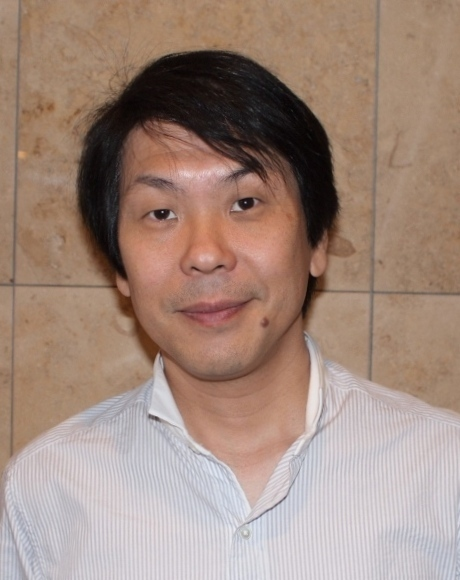
\includegraphics[height=1.5cm]{figs/Inoue-sensei.jpg} \\ \tval{Katsumi INOUE} \\ Professor \& team leader
  \end{tabular}}\right\}\text{\tval{Inoue Laboratory}}$
  &
  $\left.\text{\begin{tabular}{c}
    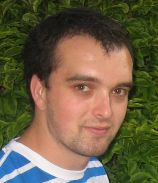
\includegraphics[height=1.5cm]{figs/Loic.jpg} \\ \tval{Loïc PAULEVÉ} \\ Post-doc
  \end{tabular}}\right\}\text{\tval{AMIB}}$
  \\ & \\ & \\
  \multicolumn{2}{l}{$\left.\text{\begin{tabular}{ccc}
      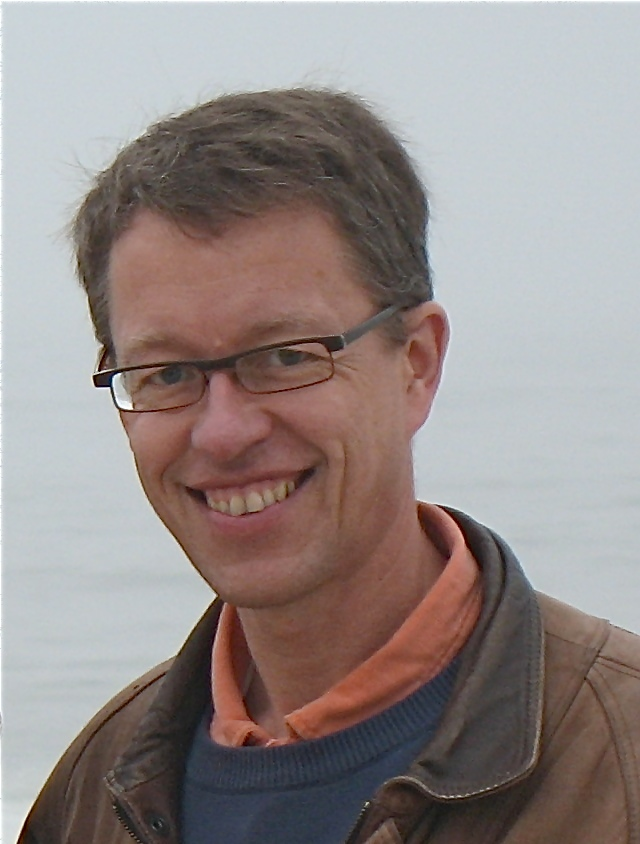
\includegraphics[height=1.5cm]{figs/Olivier.jpg}
    & 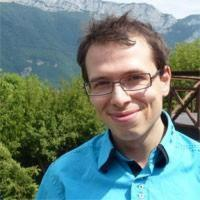
\includegraphics[height=1.5cm]{figs/Morgan.jpg}
    & 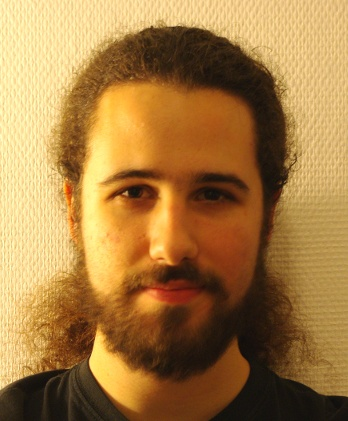
\includegraphics[height=1.5cm]{figs/Moi.jpg} \\
      \tval{Olivier ROUX} & \tval{Morgan MAGNIN} & \tval{Maxime FOLSCHETTE} \\
      Professor \& team leader & Associate professor & $\simeq$ 2\textsuperscript{nd} year PhD student
  \end{tabular}}\right\}\text{\tval{MeForBio}}$}
\end{tabular}
\end{frame}
